\chapter{Previous work - Image segmentation}\label{sec:previous-work-segmentation}
In this chapter, we will look at some of the previous work done in the field of image segmentation with neural networks. 

We will see that all of the networks presented are trained on real-world imagery and not images of maps. The reason for this being that the research is more mature in the field of real world/natural image segmentation but the same principles apply to segmentation of map images. We will also look at some of the approaches towards maps and geographical data later on in the paper.

During the last ten years, we have seen many important advances when it comes to the architecture of deep networks for image segmentation. AlexNet \cite{Krizhevsky2012}, VGGNet \cite{Simonyan2014a}, GoogLeNet \cite{Szegedy2014}, ResNet \cite{He2015}, ReNet \cite{Visin2015} and the very recent CapsNet \cite{Sabour2017} are all examples of such advances. In the next section, we will look at the main points from each of these networks.

\section{Important architectures}\label{sec:important-architectures}

TODO MAYBE LENET HERE?

TODO ZF NET?? DECONV

\subsection{AlexNet}
Achieving first place in the ImageNet Large Scale Visual Recognition Challenge (ILSVRC) \cite{Russakovsky2015}  in 2012 with a top-5 test accuracy of 84.6\% by a margin of 10\% to the next competitor, AlexNet pioneered deep CNNs in image classification. The network consisted of a total of eight-layer, five convolutional layers with max-pooling and three fully-connected layers. All the layers used ReLU as activation. To reduce overfitting they used dropout. \autoref{fig:alexnet} shows the architecture of the network.

\begin{figure}[H]
	\centering
	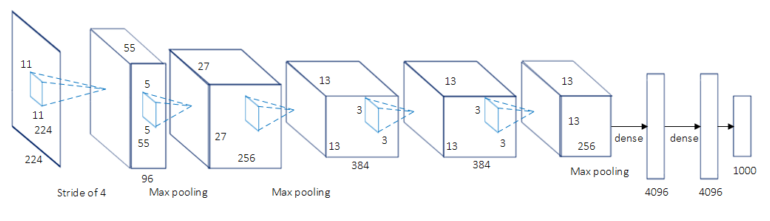
\includegraphics[width=0.7\linewidth]{fig/alexnet.png}
	\captionsource{AlexNet architecture}{\citeauthor{Krizhevsky2012}\cite{Krizhevsky2012}}
	\label{fig:alexnet}
\end{figure}


\subsection{VGG}
The Visual Geometry Group (VGG) model was introduced by the Visual Geometry Group at oxford university. In their paper, they propose multiple different architectural configurations with weight layers ranging from 13 - 16 layers deep. The most interesting is the model with 16 weight layers. It was submitted to ILSVRC 2013 and managed to get a top-5 test accuracy of 92.7\%. In \autoref{fig:vgg} we can see that the architecture makes us of more layers with small receptive fields rather than a few layers with large receptive fields.

\begin{figure}[H]
	\centering
	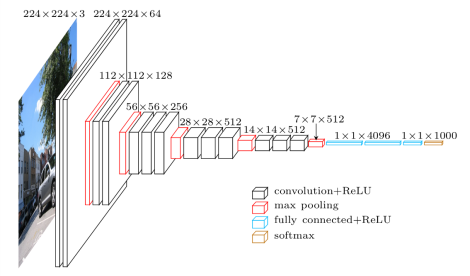
\includegraphics[width=0.7\linewidth]{fig/vgg16.png}
	\captionsource{VGG 16 architecture}{https://blog.heuritech.com/2016/02/29/a-brief-report-of-the-heuritech-deep-learning-meetup-5/}
	\label{fig:vgg}
\end{figure}


\subsection{GoogLeNet}
This network won the 2014 ILSVRC challenge with a top-5 test accuracy of 93.3\%. The network introduced a new architectural concept called the \emph{inception} model (see \autoref{fig:inceptionmodule}). The model is essentially a new mini-network with a pooling operation, large convolution layers, and smaller convolution layers. They proposed the use of small 1x1 convolution layers to reduce the complexity before the large convolution layers to keep the parameters and computational cost under control. This showed an increase in speed ranging from 3-10x faster than similar networks without the inception module.

\begin{figure}[H]
	\centering
	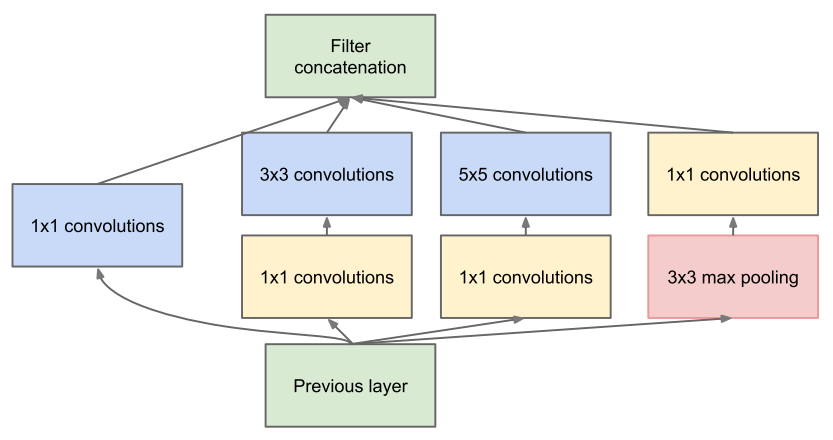
\includegraphics[width=0.7\linewidth]{fig/googlenet.png}
	\captionsource{Inception module}{\citeauthor{Szegedy2014}\cite{Szegedy2014}}
	\label{fig:inceptionmodule}
\end{figure}


\subsection{ResNet}\label{subsection:resnet}
ResNet won the 2015 ILSVRC, with a top-5 test accuracy of 96.4\%. The network is known for its depth of 152 layers and a new kind of building block called residual block. The residual block contains two paths between the input and the output where one of the paths serve as a shortcut connection to the output (see \autoref{fig:residualblock}) essentially copying the input to the output layer. A big problem with very deep networks is that they are hard to optimize. When the depth of the network increases, the accuracy gets saturated. This is called \emph{degradation} and is the problem that the residual blocks are addressing by forcing the network to learn on top of already available input. 

\begin{figure}[H]
	\centering
	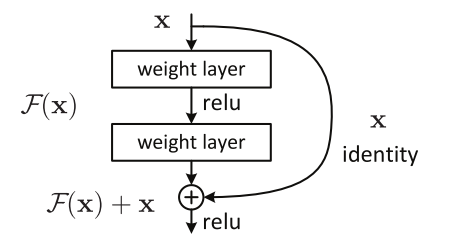
\includegraphics[width=0.5\linewidth]{fig/residual.png}
	\captionsource{Residual block.}{\citeauthor{He2015}\cite{He2015}}
	\label{fig:residualblock}
\end{figure}


\subsection{CapsNet}
Released November 2017, this is a very recent advancement in neural networks. It introduces a new type of neural network based on \emph{capsules}. 

BLABLABLA MORE ABOUT THIS

It addresses the issue that CNNs are not good at generalizing new viewpoints. They are good at generalizing to translation, but other affine transformations have shown to be difficult to learn. 


It has not (yet) been tested in ILSVRC but has been run on the Modified Institute of Standards and Technology database (MNIST) that is a database of handwritten digits. The database has 60000 training images and 10000 test images. 

\begin{figure}[H]
	\centering
	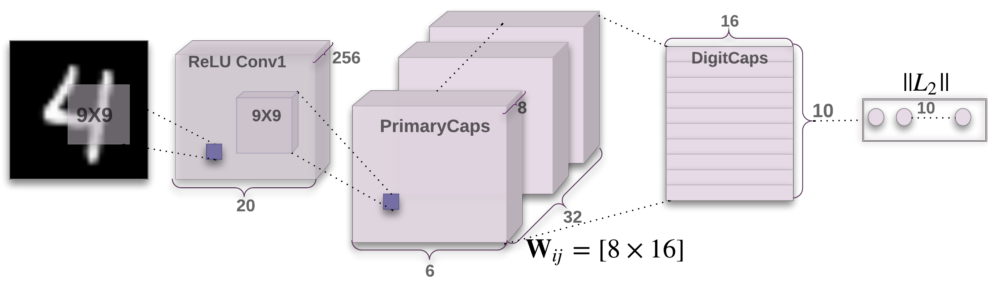
\includegraphics[width=0.7\linewidth]{fig/capsnet.png}
	\captionsource{CapsNet with 3 layers.}{\citeauthor{Sabour2017}\cite{Sabour2017}}
	\label{fig:capsnet}
\end{figure}


\section{Image segmentation}
Many of the previous network architectures described in \autoref{sec:important-architectures} are predicting labels of what the images contain and not where and what part of the image the labels are to be found in. Image segmentation is about assigning a class to each pixel with its enclosing object, also called dense predictions, so we need output from the networks that are spatial maps instead of classification scores. In this section, we will review important networks that are specialized in image segmentation. A benchmark often used for image segmentation is the PASCAL Visual Object Classes Challenge (VOC) \cite{Everingham2010}, that provides standardised image data sets for object class recognition. We will therefore evaluate the networks with the scores in VOC when applicable.


\subsection{FCN}
Fully Convolutional Network (FCN) by \citeauthor{Long2014} \cite{Long2014} can be seen as a common forerunner for semantic segmentation with convolutional networks \cite{Garcia-Garcia2017}. FCN adopted the contemporary deep classification nets AlexNet, VGG and GoogLeNet architectures we saw in \autoref{sec:important-architectures} to make dense predictions at the pixel level. It is important to note that they not only reused the architecture but used the pre-trained classification models as a starting point. The network replaced the fully-connected layers with convolutional ones, noting that the fully-connected layers could be seen as convolutional ones with kernels (filters) that cover the entire input region. This allowed segmentation maps to be generated from images of any size. Because of all the pooling operations in CNNs, a technique called \emph{deconvolution} \cite{Zeiler2011} was used to upsample the coarse output to dense pixels. Deconvolutional layers can learn interpolation functions the same way the network learns weights. Skip connections similar to the ones we saw in ResNet, are also included to give the deeper layers higher resolution feature maps. It reached a score of 62.2 in the VOC2012 challenge. 


\subsection{SegNet}
SegNet by \citeauthor{Badrinarayanan2015} \cite{Badrinarayanan2015} uses an Encoder-Decoder architecture. One can also view FCN as this type of architecture, where the downsampling is the encoding part and the deconvolution is the decoder part. The difference between these networks is in the decoding part of the architecture. In SegNet more shortcut connections are added, however instead of copying the input to the output of one layer, each upsampling layer corresponds to a max-pooling layer in the encoding part and the indices from the max-pooling layer is copied to the upsampling layer. This can be seen in \autoref{fig:segnet} where we see the blue lines as shorcut connections to the upsampling layers. The network was not benchmarked on VOC2012 in the paper but the leaderboard \cite{PASCALVOC2012a} shows that it reached a score of 59.9. 

\begin{figure}[H]
	\centering
	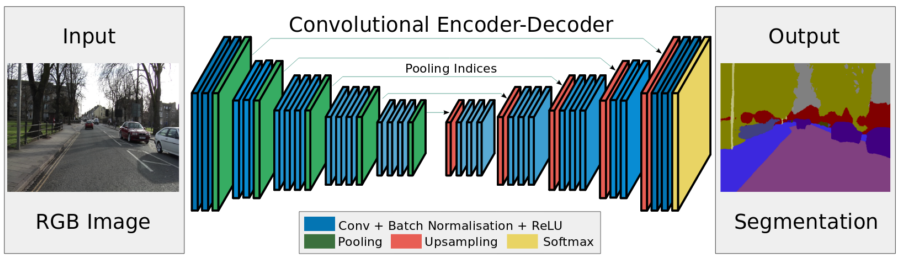
\includegraphics[width=0.7\linewidth]{fig/segnet.png}
	\captionsource{SegNet architecture.}{\citeauthor{Badrinarayanan2015}\cite{Badrinarayanan2015}}
	\label{fig:segnet}
\end{figure}


\subsection{Dilated Convolutions}
A problem with pooling layers is that they remove more context and resolution from the image the deeper we get into the network. For segmentation we need contextual reasoning and full-resolution output \cite{Yu2015}. \citeauthor{Yu2015} \cite{Yu2015} try to solve this problem with dilated convolution layers. Dilated convolution layers can increase the receptive field of a convolutional filter exponentially while the number of parameters grow linearly. This is illustrated in \autoref{fig:dilution} where we see that the receptive field, indicated in green, grows expoentially compared to the parameters, indicated as red dots. The network showed state-of-the-art perfomance with a simpler architecture, based on VGG-16 \cite{Simonyan2014a}, than the competition, scoring 71.3 in VOC2012 with their basic network.

\begin{figure}[H]
	\centering
	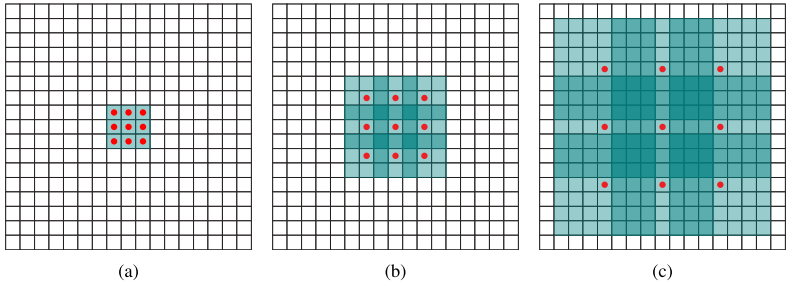
\includegraphics[width=0.7\linewidth]{fig/dilution.png}
	\captionsource{Diluted filters. (a) 1-dialted, (b) 2-dialated, (c) 3-dialated.  }{\citeauthor{Yu2015}\cite{Yu2015}}
	\label{fig:dilution}
\end{figure}


\subsection{DeepLab (v1 \& v2)}
DeepLab v1 (2014) \cite{Chen2014} and DeepLab v2 (2016) \cite{Chen2016} both used dilated convolutions though they refer to them as \emph{atrous convolutions}. They use fully-connected Conditional Random Fields (CRF) to capture fine-grained details in images as proposed by \citeauthor{Krahenbuhl2012a} \cite{Krahenbuhl2012a}. CRF can be used to combine the class scores from deep CNNs with the low-level information captured by the local interactions of pixels and edges \cite{Chen2014} and is used in DeepLab v1 as a post-processing method. As we can see in \autoref{fig:deeplab1} the effect of using CRF is significant in regards to detecting details in the image. DeepLab v1 used VGG-16 as a starting point for their architecture and got a score of 71.6 at VOC2012 beating the runner-up by a margin of 7.2\%. 

\begin{figure}[H]
	\centering
	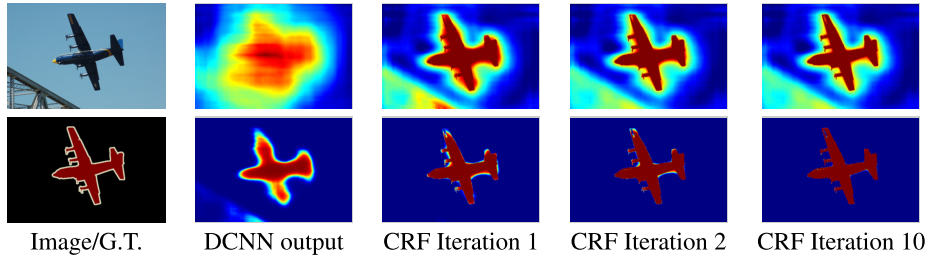
\includegraphics[width=0.7\linewidth]{fig/deeplab1.png}
	\captionsource{Score map (input before softmax) and belief map (output after softmax).  }{\citeauthor{Chen2014}\cite{Chen2014}}
	\label{fig:deeplab1}
\end{figure}


Deep CNNs can represent different object scales by training on datasets that contain objects of varying size. However explicitly accounting for scale can improve the networks ability to handle large and small objects \cite{Papandreou2015}. DeepLab v2 introduces a new technique to handle multivariate scale, called \emph{atrous spatial pyramid pooling} (ASPP). It uses multiple parallel atrous convolutional layers with different sampling rate/direction to improve the networks ability to deal with objects of different scale. DeepLab v2s best architecture used a pre-trained ResNet-101 (ResNet seen in \autoref{subsection:resnet}, that has 101 layers) with atrous convolutions, ASSP, and CRF that got a score of 79.7 at VOC2012.


\subsection{DeepLab v3}
In DeepLab v3 \cite{Chen2017a}, \citeauthor{Chen2017a} introduce an improved model of ASSP that involves concatenation of image-level features, a 1x1 convolution and three 3x3 atrous convolutions with different rates as seen in \autoref{fig:deeplab3}.

They also found it important to train with \emph{batch normalization} \cite{Ioffe2015}. A problem that occurs when when training normalized data (MAYBE EXPLAIN) is that the weights and parameters sometimes change the data som much that it becomes too big.


\begin{figure}[H]
	\centering
	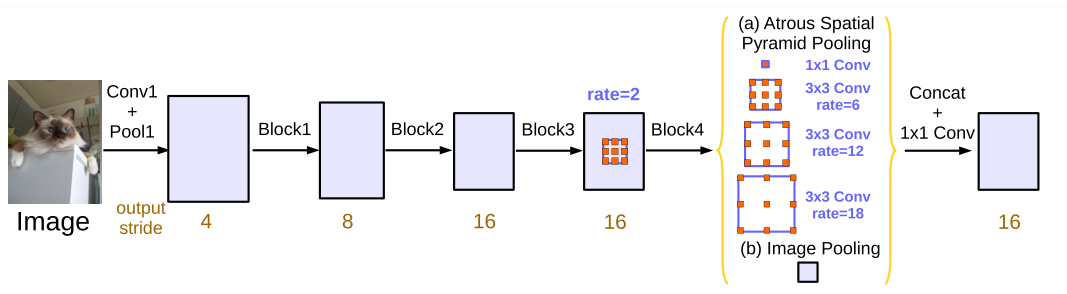
\includegraphics[width=\linewidth]{fig/deeplab3.png}
	\captionsource{Improved version of ASSP, augmented with image-level features.  }{\citeauthor{Chen2017a}\cite{Chen2017a}}
	\label{fig:deeplab3}
\end{figure}



